\section{Vorlesung 20.04.2016}

\subsection{Mechanorezeptoren von C. elegans}
\begin{itemize}
	\item 302 Neurone + 56 gliaähnlihce Zellen + 601 übrige Zellen = 959 Zellen gesamt + Keimbahn
	\item 6 Mechanorezeptoren (3 AVM (Anterior Ventral Microtubule-cell), 3 PVM (Posterior Ventral Microtubule-cell). PVM nicht funktionell. AVM hat Synapsen zu Motorneuronen. Bei Verschiebung an andere Position wird PVM funktionelle bzw. AVM nicht funktionell -$>$ keine rein zellautonome Entwicklung
	\item Fluchtreaktion nach mechanischem Stimulus (nach Mutagenese nicht mehr) -$>$ aber Kontrollversuch „Bewegung nach nicht-mechanischem Stimulus“ notwendig
	\item 350 Mutanten. Mutation in 18 Genen. Ca. 20 Allele / Gen. Keine Genkomplexe. Mutation betrifft immer alle 6 Zellen.
\end{itemize}

\textbf{Klassifikation der Mutationen:}
\begin{itemize}
	\item Zellstammbaumdefekte
	\item Determinationsdefekte
	\item Störung des sensorischen Transduktionsprozesses
	\item Spezifischer Zelltod
	\item Konnektivitätsdefekte
\end{itemize}

\subsection{Entwicklung von Nervensystemen (Neurogenese)}
Neuronale Stammzelle (Neuroblast) -$>$ Ganglienmutterzelle -$>$ Differenzierte Zelle (Neuron)\\
Kein Exponentielles Wachstum. Inäquale Teilung der Ganglienmutterzellen, so dass Neuronen unterschiedliche Komponenten bekommen\\
\\
Das \underline{Neuroektoderm} ist eine in der Embryonalentwicklung aus dem äußeren Keimblatt (Ektoderm) hervorgehende Bildung. Aus ihm entwickelt sich über das Neuroepithel des Neuralrohrs das zentrale, und über die Neuralleisten auch das periphere Nervensystem.\\

\underline{Oogenese}, auch Ovogenese, von lat. ovum, das Ei, ist die Entwicklung einer befruchtungsfähigen Eizelle (Ovum) aus einer Zelle der Keimbahn bei mehrzelligen Tieren.

Entdeckt wurden diese Gene anhand der Antennapedia-Mutation eines \underline{homöotische Gens} bei dem Modellorganismus Drosophila melanogaster, bei der am Fliegenkopf anstelle von Antennen Beine wachsen. Es handelt sich dabei um Gene, die regulatorische Proteine codieren.

\subsection{Zellautonome vs. induktive Entwicklung}
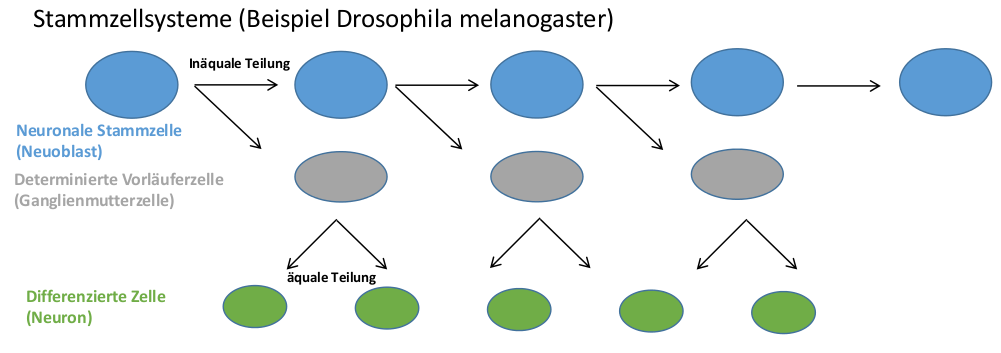
\includegraphics[width=1\textwidth]{lectures/160420/pix/stammzellsystem.png}
\\\\
keine exponentielles Wachstum, über die Zeit lineare Regulation der Zellpopulation (\textcolor{red}{\textbf{was gibt es noch dazu?}}) 